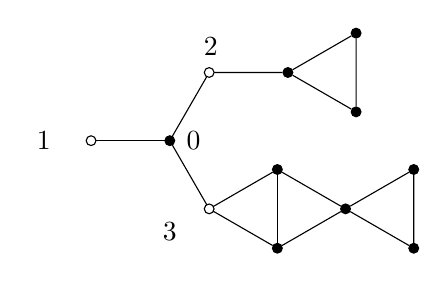
\begin{tikzpicture}[
  label distance=-5.5pt,
  thin,
  vertex/.style={circle,draw=black,fill=black,inner sep=1.25pt,
    minimum size =0mm},
  attach/.style={circle,draw=black,fill=white,inner sep=1.25pt,
    minimum size =0mm},
  dots/.style={circle,fill=black,inner sep=.5pt,
    minimum size= 0pt}]

\begin{scope}[yshift = .866cm, xshift = .5cm,rotate=0]

  \node (b) at (1,0) [vertex] {};
  \node (c) at (1.866,.5) [vertex] {};
  \node (d) at (1.866,-.5) [vertex] {};
  
  \draw (0,0) -- (b) -- (c) -- (d) -- (b);
\end{scope}

\begin{scope}[yshift = -.866cm, xshift = .5cm,rotate= -90]
  \node (e) at (.5,.866) [vertex] {};
  \node (f) at (-.5,.866) [vertex] {};
  \node (g) at (0,1.732) [vertex] {};
  \node (h) at (.5,2.598) [vertex] {};
  \node (i) at (-.5,2.598) [vertex]{};
  
  \draw (0,0) -- (e) -- (g) -- (h) -- (i) -- (g) -- (f) -- (0,0);
  \draw (e) -- (f);

\end{scope}

%%%%%%%
% Center stuff
\foreach \t in {60, 180, 300}{
  \draw (0,0) -- (\t:1);
}

\node (0) at (0,0) [vertex] {};
\node (1) at (180:1) [attach] {};
\node (2) at (60:1) [attach]{};
\node (3) at (-60:1) [attach]{};

\node at (0:.3) {$0$};
\node at (-1.6,0) {$1$};
\node at (0.52,1.2) {$2$};
\node at (0,-1.15) {$3$};

\end{tikzpicture}